%% LyX 2.0.0 created this file.  For more info, see http://www.lyx.org/.
%% Do not edit unless you really know what you are doing.
\documentclass[english,traditabstract]{aa}
\usepackage[varg]{txfonts}
%\usepackage[english,brazilian]{babel}
\usepackage[T1]{fontenc}
\setcounter{tocdepth}{3}
\usepackage{prettyref}
\usepackage{array}
\usepackage{rotating}
\usepackage{float}
\usepackage{multirow}
\usepackage{amstext}
\usepackage{graphicx}
\usepackage{epstopdf}
\usepackage{subfigure}
\usepackage{gensymb}
\usepackage{longtable}
%\usepackage{setspace}
%
%\usepackage{etoolbox}
%\AtBeginEnvironment{longtable}{\singlespacing}
%\setlength{\LTcapwidth}{\linewidth}


\makeatletter

%%%%%%%%%%%%%%%%%%%%%%%%%%%%%% LyX specific LaTeX commands.
%% Because html converters don't know tabularnewline
\providecommand{\tabularnewline}{\\}

%%%%%%%%%%%%%%%%%%%%%%%%%%%%%% User specified LaTeX commands.
\usepackage{natbib,twoopt}
\usepackage[breaklinks=true]{hyperref} %% to avoid \citeads line fills
\usepackage{arydshln}
\bibpunct{(}{)}{;}{a}{}{,} %% natbib format for A&A and ApJ
\makeatletter
\newcommandtwoopt{\citeads}[3][][]{\href{http://adsabs.harvard.edu/abs/#3}%
{\def\hyper@linkstart##1##2{}%
\let\hyper@linkend\@empty\citealp[#1][#2]{#3}}}
\newcommandtwoopt{\citepads}[3][][]{\href{http://adsabs.harvard.edu/abs/#3}%
{\def\hyper@linkstart##1##2{}%
\let\hyper@linkend\@empty\citep[#1][#2]{#3}}}
\newcommandtwoopt{\citetads}[3][][]{\href{http://adsabs.harvard.edu/abs/#3}%
{\def\hyper@linkstart##1##2{}%
\let\hyper@linkend\@empty\citet[#1][#2]{#3}}}
\newcommandtwoopt{\citeyearads}[3][][]%
{\href{http://adsabs.harvard.edu/abs/#3}
{\def\hyper@linkstart##1##2{}%
\let\hyper@linkend\@empty\citeyear[#1][#2]{#3}}}
\makeatother
\titlerunning{Astrometric Positions of the Irregular Satellites of Giant Planets}
\authorrunning{Gomes-Júnior et al.}

\makeatother


\begin{document}

\title{Astrometric positions for 18 irregular satellites of giant planets from 23 years of observations
\fnmsep\thanks{Table 8 are only available in electronic form
at the CDS via anonymous ftp to cdsarc.u-strasbg.fr (130.79.128.5)
or via http://cdsweb.u-strasbg.fr/cgi-bin/qcat?J/A+A/ and IAU NSDC data base at www.imcce.fr/nsdc.}
%\fnmsep\thanks{The complete version of Table 8 is available through CDS and IAU NSDC data base at www.imcce.fr/nsdc.}
\fnmsep\thanks{Partially based on observations made at Laborat\'orio Nacional de Astrof\'{\i}sica (LNA), Itajub\'a-MG, Brazil.}
\fnmsep\thanks{Partially based on observations through the ESO runs 079.A-9202(A), 075.C-0154, 077.C-0283 and 079.C-0345.}
\fnmsep\thanks{\textbf{Partially based on observations made at
Observatoire de Haute Provence (OHP), F-04870 Saint-Michel l'observatoire, France}}
}

\author{ A. R. Gomes-Júnior
          \inst{1},
          M. Assafin 
          \inst{1} \fnmsep\thanks{Affiliated researcher at Observatoire de Paris/IMCCE, 77 Avenue Denfert Rochereau 75014 Paris, France},
          R. Vieira-Martins
          \inst{1,2,3} \fnmsep\thanks{Affiliated researcher at Observatoire de Paris/IMCCE, 77 Avenue Denfert Rochereau 75014 Paris, France},
          J.-E. Arlot
          \inst{4},      
          J. I. B. Camargo
          \inst{2,3},     
          F. Braga-Ribas
          \inst{2,5}, 
          D. N. da Silva Neto
          \inst{6},
          A. H. Andrei
          \inst{1,2} \fnmsep\thanks{Affiliated researcher at Observatoire de Paris/SYRTE, 77 Avenue Denfert Rochereau, 75014 Paris, France},
          A. Dias-Oliveira
          \inst{2},
          B. E. Morgado
          \inst{1},
          G. Benedetti-Rossi
          \inst{2},
          Y. Duchemin
          \inst{4,7},
          J. Desmars
          \inst{4},
          V. Lainey
          \inst{4},
          W. Thuillot
          \inst{4}
          }

\offprints{A. R. Gomes-Júnior}

   \institute{Observatório do Valongo/UFRJ, Ladeira Pedro Antônio 43,
CEP 20.080-090 Rio de Janeiro - RJ, Brazil\\
              \email{altair08@astro.ufrj.br}
              \and
Observatório Nacional/MCT, R. General José Cristino 77,
CEP 20921-400 Rio de Janeiro - RJ, Brazil\\
              \email{rvm@on.br}
              \and
Laboratório Interinstitucional de e-Astronomia - LIneA, Rua Gal. José Cristino 77, Rio de Janeiro, RJ 20921-400, Brazil
              \and
Institut de mécanique céleste et de calcul des éphémérides - Observatoire de Paris, UMR 8028 du CNRS,
77 Av. Denfert-Rochereau, 75014 Paris, France\\
              \email{arlot@imcce.fr}
              \and
Federal University of Technology - Paraná (UTFPR / DAFIS), Rua Sete de Setembro, 3165, CEP 80230-901, Curitiba, PR, Brazil
              \and
Centro Universitário Estadual da Zona Oeste, Av. Manual Caldeira de Alvarenga 1203, CEP 23.070-200 Rio de Janeiro RJ, Brazil
              \and
              ESIGELEC-IRSEEM, Technopôle du Madrillet, Avenue Galilée, 76801 Saint-Etienne du Rouvray, France
              }



\date{Received ; accepted }


\abstract
{The irregular satellites of the giant planets are believed to have been captured during the evolution of the solar system. Knowing their physical parameters, such as size, density and albedo is important to constrain where they came from and how they were captured. The best way to obtain these parameters are observations in situ by spacecrafts or from stellar occultations by the objects. Both techniques demand that the orbits are well known.}
{We aimed to obtain good astrometric positions of irregular satellites in order to improve their orbits and ephemeris.}
{We identified and reduced observations of several irregular satellites from three databases containing more than 8000 images obtained between 1992 and 2014 at three sites (Observatório do Pico dos Dias, Observatoire de Haute-Provence and European Southern Observatory - La Silla).  We used the software PRAIA (Platform for Reduction of Astronomical Images Automatically) to make the astrometric reduction of the CCD frames. The UCAC4 catalogue represented the International Celestial Reference System in the reductions. The identification of the satellites in the frames was done through their ephemerides as determined from the SPICE/NAIF kernels. Some procedures were taken to overcome missing or incomplete information (coordinates, date), mostly for the older images.}
{We managed to obtain more than 6000 positions for 18 irregular satellites, being 12 of Jupiter, 4 of Saturn, 1 of Uranus (Sycorax) and 1 of Neptune (Nereid). For some satellites the number of obtained positions is more than 50\% of that used in earlier orbital numerical integrations.}
{Comparison of our positions with recent JPL ephemeris suggests the presence of systematic errors in the orbits for some of the irregular satellites. The most evident case was an error in the inclination of Carme.}


\keywords{Astrometry - Planets and satellites: general - Planets and satellites: individual: Jovian and Saturnian irregular satellites}

\maketitle

\section{Introduction} \label{Sec: introducao} 

The irregular satellites of the giant planets are smaller than the regular moons, having more eccentric, inclined, distant and, in most cases, retrograde orbits. Due to their orbital configurations, it is largely accepted that these objects were captured in the early solar system \citep{Sheppard2003}.

Because they are faint, the majority of these objects was discovered only in the last century\footnote{Website: http://ssd.jpl.nasa.gov/?sat\_discovery} . They were never visited by a spacecraft, with the exception of Himalia, Phoebe and Nereid, in a flyby by the Cassini space probe in 2000 for Himalia \citep{Porco2003} and in 2004 for Phoebe \citep{Desmars2013} and in a flyby by the Voyager 2 space probe in 1989 for Nereid \citep{Smith1989}. Even in situ, they were still opportunity target observations resulting in not optimal measurements, with size errors of $10 km$ for Himalia and $25 km$ for Nereid \citep{Thomas1991}. The exception is Phoebe with a very accurate measurement of size with a mean radius error of $0.7 km$ \citep{Thomas2010}.

%There is a number of capture mechanisms of objects by giant planets proposed in the literature. There is the Gas Drag in the primordial circumplanetary nebulae \citep{Sheppard2006} where the object would be affected by the gas drag and its velocity slowed down until it be captured by the planet. Another mechanism is called pull-down capture \citep{Sheppard2006}, where the mass of the planet would increase while the object was temporarily captured. 

%A mechanism based in the Nice model \citep{Morbidelli2005, Tsiganis2005, Gomes2005} was proposed by \citealp{Nesvorny2007} and, in the specific case of Jupiter with the modern Nice model, by \citealp{Nesvorny2014}. During the early solar system instability, encounters between the outer planets occurred. These planetary encounters could exchange energy and angular momentum between planets and the objects nearby making it possible for the capture of irregular bodies by the giant planets. In this scenario, the survival rate of prior-LHB (Late Heavy Bombardment) satellites is very small.

%Another important mechanism is the capture through collisional interactions \citep{Sheppard2006}. A collision between two small bodies in the Hill's sphere of the planet could generate fragmented objects and the dissipated energy could be such that some of these objects could be captured.

%Some of these objects are in dynamical groups with similar orbital elements, called families, similar to families found in the Main Asteroid Belt. These families may have been created by a parent body disrupted by collisions with comets or other satellites \citep{Nesvorny2004}. Collisions with comets are more likely to have occurred during the Late Heavy Bombardment (LHB) \citep{Gomes2005}.

%\citealp{Nesvorny2003} studied the collision rates between irregular satellites and concluded that some satellites could have been removed by collision with a bigger satellite. The rate collision between satellites of the Himalia Group (Himalia, Elara, Lysithea and Leda, mainly), for instance, was found to be more than one during the solar system age suggesting that their current structure was originated by satellite-satellite collision.

%For Phoebe, ejected material from its surface caused by impacts could evolve due to Poynting-Robertson drag and collide with Iapetus causing the large variation in albedo observed on it \citep{Nesvorny2003}. Indeed, Cassini was able to detected in Phoebe an absorption feature at 2.42 $\mu m$ (probably CN combinations) that was also detected in the dark side of Iapetus \citep{Clark2005}.

If these objects were captured, there remains the question of where they came from. \citealp{Clark2005} showed from imaging spectroscopy from Cassini that Phoebe has a surface probably covered by material from the outer solar system and \citealp{Grav2003} showed that the satellites of the Jovian Prograde Group Himalia have grey colors implying that their surfaces are similar to that of C-type asteroids. In that same work, the Jovian Retrograde Group Carme was found to have surface colors similar to the D-type asteroids like Hilda or Trojan families while JXIII Kalyke has a redder color like Centaurs or trans-neptunian objects (TNOs).

For Saturnian satellites, \citealp{Grav2007} showed by their colors and spectral slopes that these satellites contain a more or less equal fraction of C-, P- and D-like objects but SXXII Ijiraq is marginally redder than D-type objects. These works may suggest different origins for the irregular satellites.

In this context, we used 3 databases for deriving precise positions for the irregular satellites observed at Observatório do Pico dos Dias (1.6 m and 0.6 m telescopes, IAU code 874), Observatoire Haute-Provence (1.2m telescope, IAU code 511) and ESO (2.2 m telescope, IAU code 809). Many irregular satellites were observed between 1992 and 2014 covering a few orbital periods of these objects (12 satellites of Jupiter, 4 of Saturn, Sycorax of Uranus and Nereid of Neptune). 

\textbf{Since their ephemerides are not very precise, predict and observe stellar occultations are very difficult and no observation of such an event for an irregular satellite is found in the literature. The precise star positions to be derived by the ESA astrometry satellite Gaia \citep{deBruijne2012} will render better predictions with the only source of error being the ephemeris. The positions derived from \textbf{our} observations can be used in new orbital numerical integrations, generating more precise ephemerides.}

\textbf{The power of stellar occultations for observing relatively small diameter solar system objects is supported by recent works such as the discovery of a ring system around the Centaur (10199) Chariklo \citep{Braga-Ribas2014}. Once irregular satellites start to be observed by this technique, it will be possible to obtain their physical parameters (shape, size, albedo, density) with unprecedented precision. For instance, in this case, sizes could be obtained with kilometer accuracy. The knowledge of these parameters would in turn bring valuable information for the study of the capture mechanisms and origin of the irregular satellites.}

The databases are described in Sect. \ref{Sec: observations}. The astrometric procedures in Sect. \ref{Sec: reduction}. The obtained positions are presented in Sect \ref{Sec: positions} and analysed in Sect. \ref{Sec: comparison}. Conclusions are given in Sect. \ref{Sec: conclusions}.


\section{Databases} \label{Sec: observations}

Our three databases consist in optical CCD images from many observational programs performed with different telescopes/detectors targeting a variety of objects, among which irregular satellites. The observations were made at 3 sites: Observatório do Pico dos Dias (OPD), Observatoire Haute-Provence (OHP) and European Southern Observatory (ESO). Altogether there are more than 8000 FITS images obtained in a large time span (1992-2014) for the irregular satellites. Since the OHP and mostly the OPD database registers were not well organized, we had to start from scratch and develop an automatic procedure to identify and filter only the images of interest, that is, of the irregular satellites. The instruments and images characteristics are described in the following subsections.

\subsection{OPD} \label{Subsec: observations-opd}

The OPD database was produced at Observatório do Pico dos Dias (OPD, IAU code 874, $45^{\circ} ~34\arcmin ~57\arcsec$ W, $22^{\circ} ~32\arcmin ~04\arcsec$ S, 1864 m)\footnote{Website: http://www.lna.br/opd/opd.html - in Portuguese}, located at geographical longitude , in Brazil. The observations were made between 1992 and 2014 by our group in a variety of observational programs. %In Fig \ref{Fig: obsxyear-opd} we plot the number of frames obtained per satellite over time and in Fig \ref{Fig: obsxsat-opd} the number of frames per satellite for each telescope. 
Two telescopes of 0.6 m diameter (Zeiss and Boller \& Chivens) and one 1.6 m diameter (Perkin-Elmer) were used for the observations. It was identified 5248 observations containing irregular satellites, being 3168 from the Boller \& Chivens, 1967 from the Perkin-Elmer and 113 from the Zeiss.

%\begin{figure*}
%\begin{centering}
%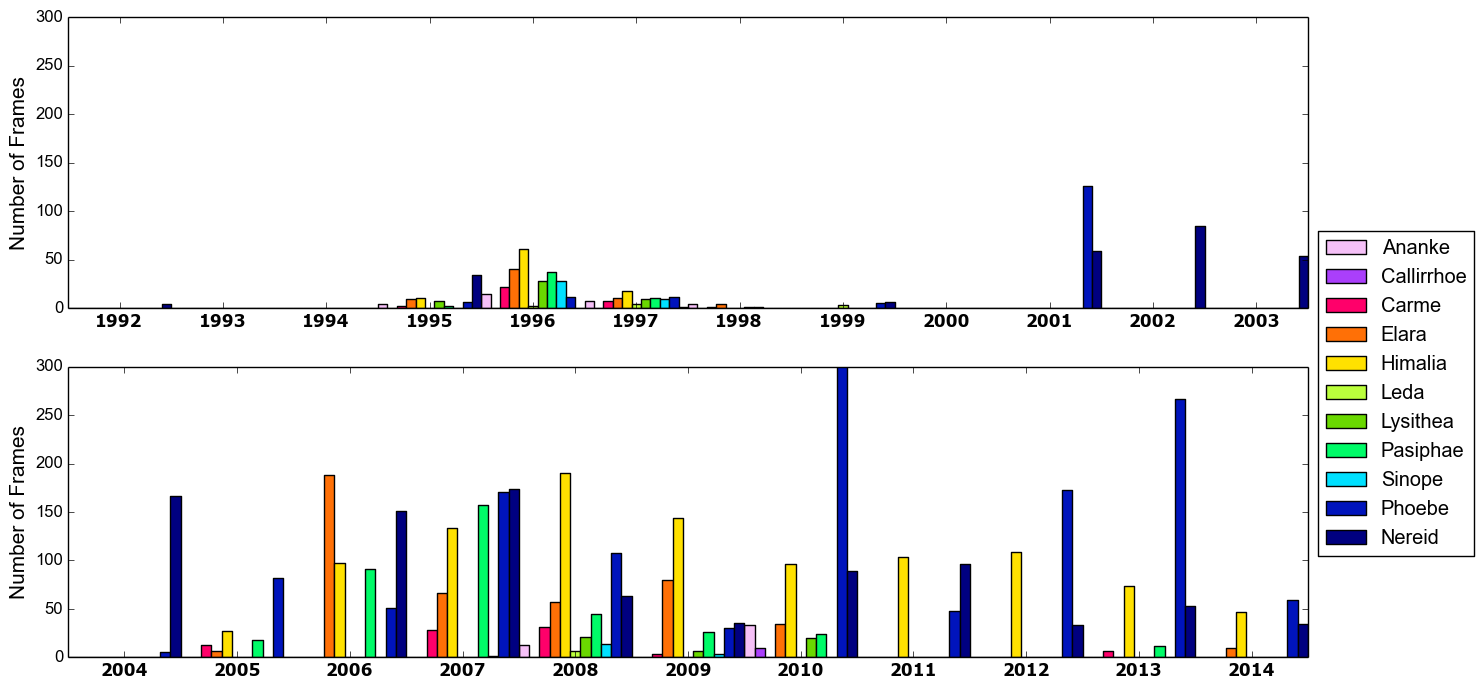
\includegraphics[width=17cm]{figures/framexobj_ano_opd}
%\par\end{centering}
%\caption{Distribution of the observations of the satellites over time at OPD. The graphic is limited in number of frames to 300 for better viewing. The number of frames of Phoebe in 2010 is 533.}
%\label{Fig: obsxyear-opd}
%\end{figure*}

This is an inhomogeneous database with observations made with 9 different detectors (see Table \ref{Tab: OPD-CCDs}) and 6 different filters. The headers of most of the older FITS images had missing, incomplete or incorrect coordinates or date. In some cases, we could not identify the detector origin. The procedures used to overcome these problems are described in Sect. \ref{Sec: reduction}.

\begin{table}[h!]
\caption{\label{Tab: OPD-CCDs} Characteristics of OPD detectors used in this work.}
\begin{centering}
\begin{tabular}{ccc}
\hline
\hline
\multicolumn{3}{c}{Perkin-Elmer}\tabularnewline
% & \multicolumn{2}{c}{Exposure Times}\tabularnewline
Detector & Image Size (pixel) & Pixel Scale ($\mu m$/px)\tabularnewline
\hline
CCD048 & 770 x 1152 & 22.5\tabularnewline
CCD098 & 2048 x 2048 & 13.5\tabularnewline
CCD101 & 1024 x 1024 & 24.0\tabularnewline
CCD105 & 2048 x 2048 & 13.5\tabularnewline
CCD106 & 1024 x 1024 & 24.0\tabularnewline
CCD301 & 385 x 578 & 22.0\tabularnewline
CCD523 & 455 x 512 & 19.0\tabularnewline
IKON & 2048 x 2048 & 13.5\tabularnewline
IXON & 1024 x 1024 & 13.5\tabularnewline
\hline 
\end{tabular} 
\par\end{centering}
The plate scale of the telescopes are 13.09"/mm for Perkin-Elmer, 25.09"/mm for Boller \& Chivens and 27.5"/mm for Zeiss.
\end{table}

%\begin{figure}
%\begin{centering}
%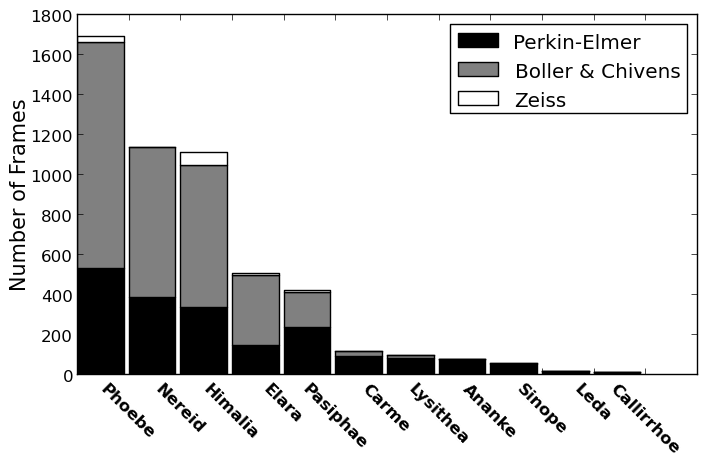
\includegraphics[scale=0.45]{figures/framexobj_opd}
%\par\end{centering}
%
%\caption{Number of frames observed per satellite by OPD telescope.}
%
%
%\label{Fig: obsxsat-opd}
%\end{figure}

\subsection{OHP} \label{Subsec: observations-ohp}

The instrument used at the Observatoire de Haute Provence (OHP, IAU code 511, $5^{\circ} ~42\arcmin ~56.5\arcsec$ E, $43^{\circ} ~55\arcmin ~54.7\arcsec $N, 633.9 m)\footnote{Website: www.obs-hp.fr/guide/t120.shtml - in French} was the 1.2m-telescope in a Newton configuration. The focal length is 7.2 m. The observations were made between 1997 and 2008. During this time only one CCD detector $1024 \times 1024$ was used. The size of field is $12\arcmin \times 12\arcmin$ with a pixel scale of $0.69\arcsec$.  %Fig. \ref{Fig: obsxyear-ohp} shows the distribution of the observation of the satellites over time and Fig. \ref{Fig: obsxsat-ohp} the number of frames observed for each satellite. 
From these observations, 2408 were identified containing irregular satellites.


%\begin{figure*}
%\begin{centering}
%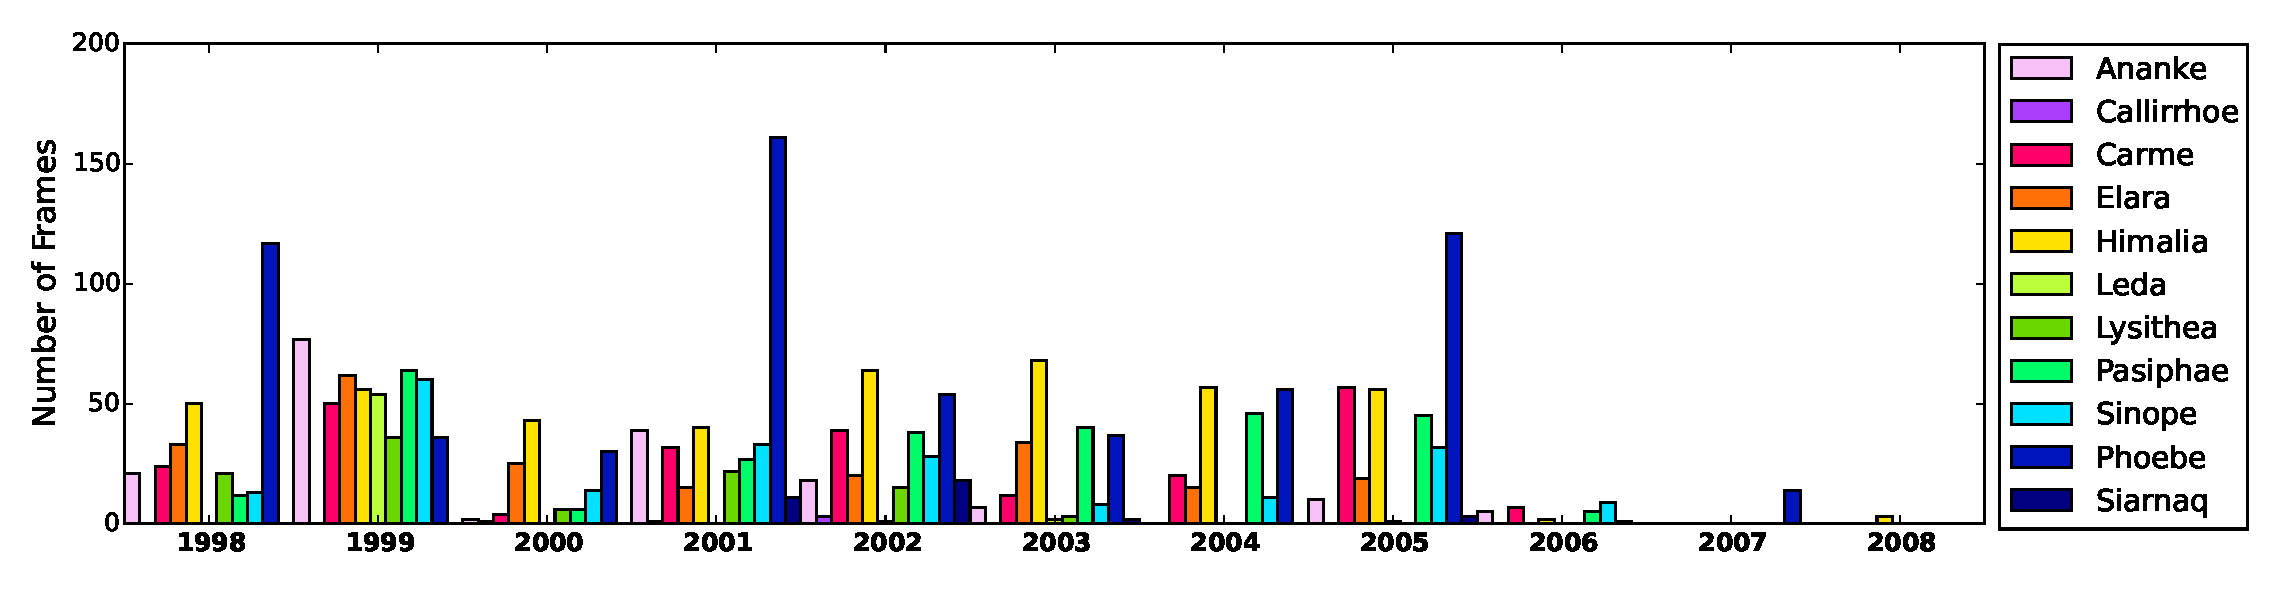
\includegraphics[scale=0.48]{figures/framexobj_ano_ohp}
%\par\end{centering}
%
%\caption{Distribution of the observations of the satellites over time from observations at OHP.}
%\label{Fig: obsxyear-ohp}
%\end{figure*}
%
%\begin{figure}
%\begin{centering}
%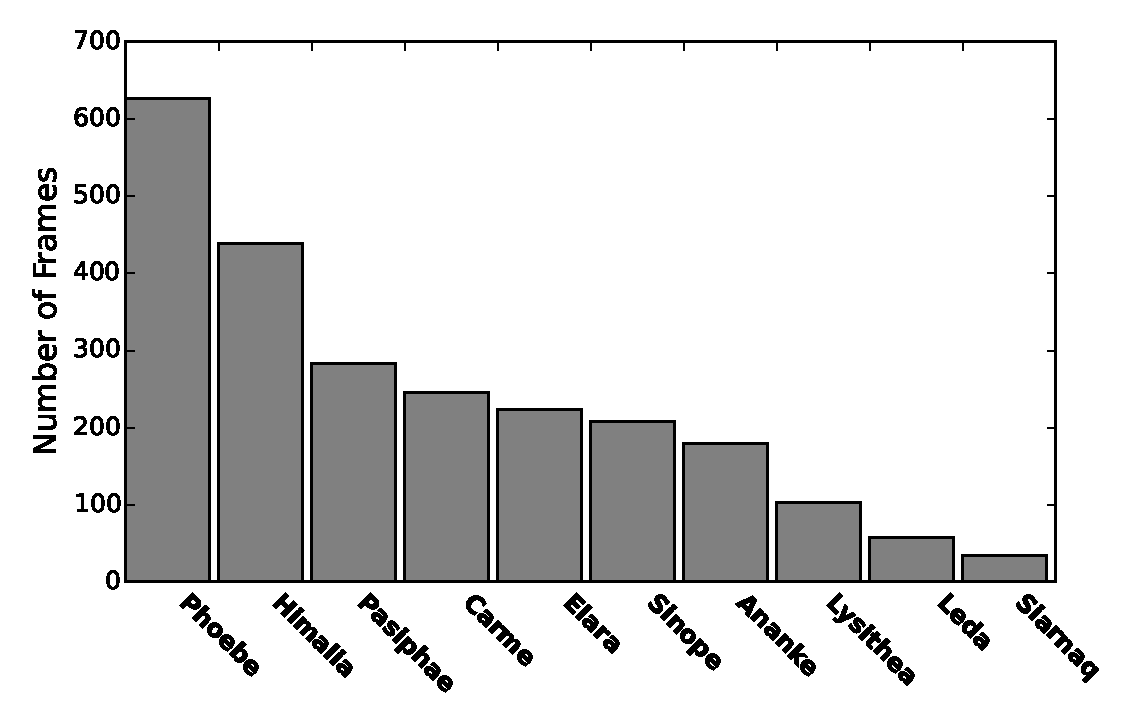
\includegraphics[scale=0.45]{figures/framexobj_ohp}
%\par\end{centering}
%
%\caption{Number of frames per satellite observed at OHP.}
%
%
%\label{Fig: obsxsat-ohp}
%\end{figure}


\subsection{ESO} \label{Subsec: observations-eso}

Observations were made at the 2.2 m Max-Planck ESO (ESO2p2) telescope (IAU code 809, $70\degr44\arcmin1.5\arcsec$ W, $29\degr15\arcmin31.8\arcsec$ S, 2345.4 m)\footnote{Website: www.eso.org/sci/facilities/lasilla/telescopes/\\national/2p2.html} with the Wide Field Imager (WFI) CCD mosaic detector. Each mosaic is composed by eight CCDs of $7.5\arcmin \times 15\arcmin$ ($\alpha$, $\delta$) sizes, resulting in a total coverage of $30\arcmin \times 30\arcmin$ per mosaic. Each CCD has $4 k \times 2 k$ pixels with a pixel scale of $0.238\arcsec$. The filter used was a broad-band R filter (ESO\#844) with $\lambda _{c}  = 651.725$ nm and $\Delta \lambda = 162.184$ nm. The telescope was shifted between exposures in such a way that each satellite was observed at least twice in different CCDs.

The satellites were observed in 24 nights, divided in 5 runs, between April 2007 and May 2009 in paralel with, and using the same observational and astrometric procedures of the program that observed stars along the sky path of trans-neptunian objects (TNOs) to identify candidates to stellar occultation \citep[see][]{2010A&A...515A..32A, 2012A&A...541A.142A}. A total of 810 observations for irregular satellites were obtained. %Fig \ref{Fig: obsxsat-eso} shows the number of frames per satellite.

%\begin{figure}
%\begin{centering}
%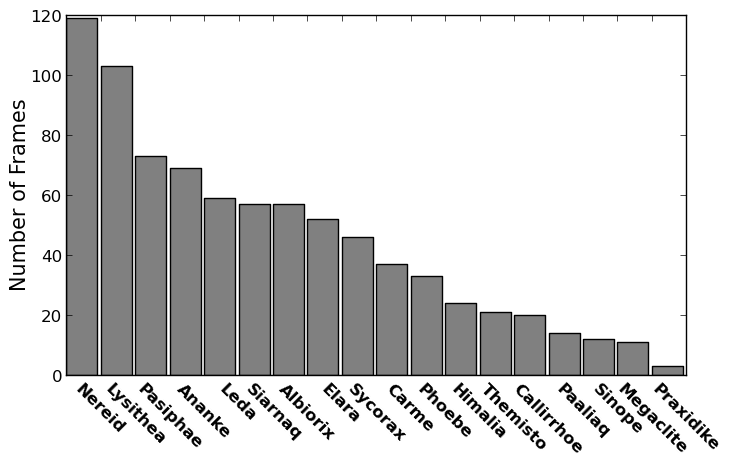
\includegraphics[scale=0.45]{figures/framexobj_eso}
%\par\end{centering}
%
%\caption{Number of frames per satellite observed at ESO.}
%
%
%\label{Fig: obsxsat-eso}
%\end{figure}

\section{Astrometry} \label{Sec: reduction}

Almost all the frames were photometrically calibrated with auxiliary bias and flat-field frames by means of standard procedures using IRAF\footnote{Website: http://iraf.noao.edu/} and, for the mosaics, using the esowfi \citep{Jones2000} and mscred \citep{Valdes1998} packages. Some of the nights at OPD didn't have bias and flat-field images so the correction was not possible.

The astrometric treatment was made with the Platform for Reduction of Astronomical Images Automatically (PRAIA) \citep{2011gfun.conf...85A}. The (x, y) measurements were performed with 2-dimensional circular symmetric Gaussian fits within one Full Width Half Maximum (FWHM = seeing). Within one FWHM, the image profile is well described by a Gaussian profile, free from the wing distortions, which may jeopardize the center determination. PRAIA automatically recognizes catalog stars and determines ($\alpha$, $\delta$) with a user-defined model relating the (x, y) measured and (X, Y) standard coordinates projected in the sky tangent plane.

We used the UCAC4 \citep{2013AJ....145...44Z} as the practical representative of the International Celestial Reference System (ICRS). For each frame, we used the six constants polynomial model to relate the (x, y) measurements with the (X, Y) tangent plane coordinates. For ESO, we followed the same astrometric procedures described in detail in \cite{2012A&A...541A.142A}; the (x, y) measurements of the individual CCDs were pre-corrected by a field distortion pattern, and all positions coming from different CCDs and mosaics were then combined using a 3rd degree polynomial model to produce a global solution for each night and field observed, and final ($\alpha$, $\delta$) object positions were obtained in the UCAC4 system. 

In Table \ref{Tab: stars-errors} we list the average mean error in $\alpha$ and $\delta$ for the reference stars obtained by telescope, the average (x, y) measurement errors of the Gaussian fits described above and the mean number of UCAC4 stars used by frame. For all databases, about 20\% of outlier reference stars were eliminated for presenting (O-C) position residuals higher than 120 mas in the ($\alpha$, $\delta$) reductions. %##### OHP = 21\% de estrelas eliminadas, erro gaussiano: média de 26mas e 90\% entre 5 e 60mas para x e y; ESO = erro gaussiano: média de 14mas e 90\% entre 2 e 41mas; 160 = 13\% de estrelas eliminadas,  média de 15mas e 90\% entre 3 e 38mas ; IAG = 24\% d estrelas eliminadas, média de 29mas e 90\% entre 3 e 75mas ; Zeiss = 37\% de estrelas eliminadas, média de 26mas e 90\% entre 5 e 56mas#####

\begin{table}
\caption{\label{Tab: stars-errors} Astrometric ($\alpha$, $\delta$) reduction by telescope.}
\begin{centering}
\begin{tabular}{lccccc}
\hline %\multicolumn{6}{c}{Perkin-Elmer} \tabularnewline
\hline
 & \multicolumn{2}{c}{Mean errors} &  UCAC4 & \multicolumn{2}{c}{Gaus. errors}       \tabularnewline
Telescope  & $\sigma_{\alpha}$  & $\sigma_{\delta}$  & stars & x & y  \tabularnewline
  &   mas   &   mas & &   mas   &   mas  \tabularnewline
\hline
PE(OPD) & 51 & 48 & 24 & 15 & 15 \tabularnewline
B\&C (OPD) & 56 & 55 & 36 & 29 & 29 \tabularnewline
Zeiss (OPD) & 58 & 57 & 95 & 26 & 26 \tabularnewline
OHP & 50 & 49 & 46 & 26 & 26 \tabularnewline
ESO & 26 & 25 & 632 & 15 & 15 \tabularnewline
\hline
\end{tabular}
\par\end{centering}
Mean errors are the standard deviations in the (O$-$C) residuals from ($\alpha$, $\delta$) reductions with the UCAC4 catalog. Gaussian errors are the errors in the Gaussian fit used to perform the (x, y) measurements.
\end{table}

To help identifying the satellites in the frames, and derive the ephemeris for the instants of the observations for comparisons (see Sect \ref{Sec: comparison}), we used the kernels from SPICE/JPL\footnote{Website: http://naif.jpl.nasa.gov/naif/toolkit.html}. \cite{Emelyanov2008} and references therein also provided ephemeris of similar quality for the irregular satellites. For instance, for Himalia, which has relatively good orbit solutions, the ephemerides differ by less than $20 mas$, and in the case of less-known orbits, like Ananke, the differences are less than $90 mas$. Here, we choose to use the JPL ephemeris because they used more recent observations \cite[see][]{Jacobson2012}. The JPL ephemeris that represented the Jovian satellites in this work was the DE421 $+$ JUP300. For the Saturnian satellites the ephemeris was DE421 $+$ SAT359 to Hyperion, Iapetus and Phoebe and DE421 $+$ SAT361 to Albiorix, Siarnaq and Paaliaq. The DE421 $+$ URA095 was used for Sycorax and DE421 $+$ NEP081 for Nereid. More recent JPL ephemeris versions became available after completion of this work, but this did not affect the results. 

In the OPD database, there were some images (mostly the older ones) with missing coordinates or wrong date in their headers. In the case of missing or wrong coordinates, we adopted the ephemeris as the central coordinates of the frames. When the time was not correct, the FOV identification failed. In this case, a search for wrong date (year) displaying was performed. Problems like registering local time instead of UTC were also identified and corrected.

In all databases, for each night a sigma-clipping procedure was performed to eliminate discrepant positions (outliers). A threshold of 120 mas and a deviation of more than 2.5 sigmas from the nightly average ephemeris offsets were adopted.

From Table \ref{Tab: Reductions-160} to \ref{Tab: Reductions-eso} we list the average dispersion (standard deviation) of the position offsets with regard to the ephemeris for $\alpha$ and $\delta$ obtained by telescope for each satellite. The final number of frames, number of nights (in parenthesis), the mean number of UCAC4 stars used in the reduction and the approximate V magnitude are also given. The dashed lines separate the satellites from different families with similar orbital parameters: Himalia Group (Himalia, Elara, Lysithea and Leda), Pasiphae Group (Pasiphae, Callirrhoe and Megaclite) and Ananke Group (Ananke and Praxidike). Carme and Sinope are the only samples of their groups. From Saturn, Siarnaq and Paaliaq are from the Inuit Group while Phoebe and Albiorix are the only samples of their groups.

The differences in the dispersion of the ephemeris offsets of the same satellite for distinct telescopes seen in Tables \ref{Tab: Reductions-160} to \ref{Tab: Reductions-eso} are caused by the different distribution of observations along the orbit for each telescope. This can be seen in Fig \ref{Fig: carme_anom} for Carme, \ref{Fig: pasiphae_anom} for Pasiphae and for all objects in the online material. Since the observations cover different segments of the orbit, the dispersion of the offsets may vary for different telescopes for a single satellite, with larger covered segments usually implying in larger dispersions and vice-versa. For Nereid, due to its high eccentric orbit, the observations are located between 90$\degree$ and 270$\degree$ of True Anomaly where Nereid remains most of the time.

\begin{table}
\caption{\label{Tab: Reductions-160} Astrometric ($\alpha$, $\delta$) reduction for each satellite observed with the Perkin-Elmer telescope.}
\begin{centering}
\begin{tabular}{lcccccc}
\hline 
%\multicolumn{6}{c}{Perkin-Elmer} \tabularnewline
\hline
 & \multicolumn{2}{c}{Offsets (sigma)} & Nr &  UCAC4 & \tabularnewline
Satellite  & $\sigma_{\alpha}$  & $\sigma_{\delta}$ & frames  & stars & Mag \tabularnewline
  &   mas   &   mas  & (nights)  & &\tabularnewline
\hline
Himalia & 290 & 45 & 238 (18) & 37 & 14 \tabularnewline
Elara & 230 & 118 & 99 (12) & 32 & 16\tabularnewline
Lysithea & 107 & 79 & 53 (8) & 41 & 18\tabularnewline
Leda & 207 & 79 & 6 (2) & 46 & 19\tabularnewline
\hdashline
Pasiphae & 157 & 92 & 144 (13) & 22 & 17 \tabularnewline
Callirrhoe & 66 & 35  &   9 (1) & 3 & 21\tabularnewline
\hdashline
Carme & 97 & 94 & 68 (7) & 49 & 18\tabularnewline
Sinope & 155 & 77 & 37 (8) & 42 & 18\tabularnewline
Ananke & 93 & 185 & 52 (7) & 40 & 19\tabularnewline
\hline
Phoebe & 73 & 95 & 410 (22) & 6 & 16\tabularnewline
\hline
Nereid & 200 & 142 & 289 (29) & 8 & 19\tabularnewline
\hline
\end{tabular}
\par\end{centering}
The offsets (sigma) are the average standard deviations of the ephemeris offsets from the ($\alpha$, $\delta$) positions of the satellites. Also given are the approximate satellite V magnitude and the average number of UCAC4 reference stars per frame.
\end{table}

\begin{table}
\caption{\label{Tab: Reductions-iag} Astrometric ($\alpha$, $\delta$) reduction for each satellite observed with the Boller \& Chivens telescope.}
\begin{centering}
\begin{tabular}{lccccc}
\hline 
%\multicolumn{6}{c}{Boller \& Chivens} \tabularnewline
\hline
 & \multicolumn{2}{c}{Offsets (sigma)} & Nr &  UCAC4 & \tabularnewline
Satellite  & $\sigma_{\alpha}$  & $\sigma_{\delta}$ & frames  & stars & Mag \tabularnewline
  &   mas   &   mas  & (nights)  & &\tabularnewline
\hline
Himalia & 83 & 43 & 560 (31) & 57 & 14 \tabularnewline
Elara & 55 & 43 & 294 (23) & 53 & 16 \tabularnewline
Lysithea & 23 & 42 & 7 (2) & 60 & 18 \tabularnewline
\hdashline
Pasiphae & 128 & 71 & 140 (14) & 57 & 17 \tabularnewline
Carme & 68 & 111 & 22 (4) & 45 & 18\tabularnewline
Sinope & 59 & 17  &   4 (1) & 22 & 18\tabularnewline
\hline
Phoebe & 43 & 48 & 810 (42) & 17 & 16 \tabularnewline
\hline
Nereid & 61 & 45 & 514 (38) & 20 & 19 \tabularnewline
\hline
\end{tabular}
\par\end{centering}
Same as in Table \ref{Tab: Reductions-160}.
%Mean errors are the standard deviations in the (O$-$C) residuals from ($\alpha$, $\delta$) reductions with the UCAC4 catalog.
\end{table}

\begin{table}
\caption{\label{Tab: Reductions-zei} Astrometric ($\alpha$, $\delta$) reduction for each satellite observed with the Zeiss telescope.}
\begin{centering}
\begin{tabular}{lccccc}
\hline 
%\multicolumn{6}{c}{Zeiss} \tabularnewline
\hline
 & \multicolumn{2}{c}{Offsets (sigma)} & Nr &  UCAC4 & \tabularnewline
Satellite  & $\sigma_{\alpha}$  & $\sigma_{\delta}$ & frames  & stars & Mag \tabularnewline
  &   mas   &   mas  & (nights)  & &\tabularnewline
\hline
Himalia & 112 & 72 & 56 (4) & 91 & 14\tabularnewline
Elara & 17 & 21  &  10 (1) & 146 & 16 \tabularnewline
\hdashline
Pasiphae & 24 & 25  &  11 (1) & 140 & 17\tabularnewline
\hline
Phoebe & 37 & 30  &  19 (1) & 16 & 16\tabularnewline
\hline
\end{tabular}
\par\end{centering}
Same as in Table \ref{Tab: Reductions-160}.
%Mean errors are the standard deviations in the (O$-$C) residuals from ($\alpha$, $\delta$) reductions with the UCAC4 catalog.
\end{table}

\begin{table}
\caption{\label{Tab: Reductions-ohp} Astrometric ($\alpha$, $\delta$) reduction for each satellite observed with the OHP telescope.}
\begin{centering}
\begin{tabular}{lccccc}
\hline
%\multicolumn{6}{c}{OHP} \tabularnewline
\hline
 & \multicolumn{2}{c}{Offsets (sigma)} & Nr &  UCAC4 & \tabularnewline
Satellite  & $\sigma_{\alpha}$  & $\sigma_{\delta}$ & frames  & stars & Mag \tabularnewline
  &   mas   &   mas  & (nights)  & &\tabularnewline
\hline
Himalia & 49 & 66 & 357 (43) & 49 & 14\tabularnewline
Elara & 52 & 61 & 187 (25) & 37 & 16\tabularnewline
Lysithea & 63 & 50 & 84 (13) & 56 & 18\tabularnewline
Leda & 118 & 33 & 48 (7) & 14 & 19\tabularnewline
\hdashline
Pasiphae & 101 & 75 & 248 (32) & 39 & 17\tabularnewline
Carme & 114 & 96 & 204 (29) & 39 & 18\tabularnewline
Sinope & 196 & 73 & 169 (25) & 43 & 18\tabularnewline
Ananke & 100 & 89 & 141 (20) & 62 & 19\tabularnewline
\hline
Phoebe & 30 & 31 & 516 (63) & 51 & 16\tabularnewline
Siarnaq & 46 & 98 & 20 (6) & 32 & 20\tabularnewline
\hline
\end{tabular}
\par\end{centering}
Same as in Table \ref{Tab: Reductions-160}.
%Mean errors are the standard deviations in the (O$-$C) residuals from ($\alpha$, $\delta$) reductions with the UCAC4 catalog.
\end{table}

\begin{table}
\caption{\label{Tab: Reductions-eso} Astrometric ($\alpha$, $\delta$) reduction for each satellite observed with the ESO telescope.}
\begin{centering}
\begin{tabular}{lccccc}
\hline 
%\multicolumn{6}{c}{ESO} \tabularnewline
\hline
 & \multicolumn{2}{c}{Offsets (sigma)} & Nr &  UCAC4 & \tabularnewline
Satellite  & $\sigma_{\alpha}$  & $\sigma_{\delta}$ & frames  & stars & Mag \tabularnewline
  &   mas   &   mas  & (nights)  & &\tabularnewline
\hline
Himalia & 76 & 74 & 23 (2) & 1153 & 14\tabularnewline
Elara & 112 & 87 & 46 (4) & 1492 & 16\tabularnewline
Lysithea & 76 & 88 & 90 (6) & 695 & 18\tabularnewline
Leda & 60 & 125 & 44 (3) & 632 & 19\tabularnewline
\hdashline
Pasiphae & 70 & 114 & 66 (5) & 836 & 17\tabularnewline
Callirrhoe & 29 & 33  &  16 (1) & 493 & 21\tabularnewline
Megaclite & 52 & 34  &  10 (1) & 445  & 22\tabularnewline
\hdashline
Ananke & 225 & 19 & 57 (3) & 761 & 18\tabularnewline
Praxidike & 7 & 38  &   2 (1) & 1934 & 21\tabularnewline
\hdashline
Carme & 140 & 110 & 37 (4) & 1074 & 18\tabularnewline
Sinope & 339 & 70 & 11 (2) & 1542 & 18\tabularnewline
Themisto & 894 & 28 & 16 (2) & 1232 & 21\tabularnewline
\hline
Phoebe & 102 & 57 & 32 (5) & 312 & 16\tabularnewline
\hdashline
Siarnaq & 86 & 66 & 56 (6) & 283 & 20\tabularnewline
Paaliaq & 301 & 59 & 11 (4) & 382 & 21\tabularnewline
\hdashline
Albiorix & 76 & 50 & 46 (6) & 330 & 20\tabularnewline
\hline
Sycorax & 150 & 82 & 35 (9) & 375 & 21\tabularnewline
\hline
Nereid & 115 & 78 & 99 (12) & 362 & 19\tabularnewline
\hline
\end{tabular}
\par\end{centering}
Same as in Table \ref{Tab: Reductions-160}.
%Mean errors are the standard deviations in the (O$-$C) residuals from ($\alpha$, $\delta$) reductions with the UCAC4 catalog.
\end{table}


%\begin{table*}
%\caption{\label{Tab: offsets} Error by satellite by telescope}
%\begin{centering}
%\begin{tabular}{lccccccccccccccc}
%\hline\hline 
%Satellite & \multicolumn{3}{c}{Perkin-Elmer} & \multicolumn{3}{c}{Boller \& Chivens} & \multicolumn{3}{c}{Zeiss} & \multicolumn{3}{c}{OHP} & \multicolumn{3}{c}{ESO}\tabularnewline
% & $\sigma_\alpha$ & $\sigma_\delta$ & N & $\sigma_\alpha$ & $\sigma_\delta$ & N & $\sigma_\alpha$ & $\sigma_\delta$ & N & $\sigma_\alpha$ & $\sigma_\delta$ & N & $\sigma_\alpha$ & $\sigma_\delta$ & N\tabularnewline
%  & mas & mas & stars & mas & mas & stars & mas & mas & stars & mas & mas & stars & mas & mas & stars\tabularnewline
%\hline
%Ananke & 18.8 & 70 & 179 & 249 & 1995 & 600 & 1951 & 18.8 & 70 & 179 & 249 & 1995& 600 & 1951 & 0 \tabularnewline
%Callirrhoe & 20.6 & 9 & 5 & 14 & 2000 & 95 & 1999 & 18.8 & 70 & 179 & 249 & 1995 & 600 & 1951 & 0 \tabularnewline
%Carme & 17.8 & 62 & 245 & 307 & 1995 & 973 & 1938 & 18.8 & 70 & 179 & 249 & 1995 & 600 & 1951 & 0 \tabularnewline
%Elara & 16.6 & 349 & 223 & 572 & 1995 & 1115 & 1905 & 18.8 & 70 & 179 & 249 & 1995 & 600 & 1951 & 0 \tabularnewline
%Himalia & 14.6 & 645 & 444 & 1089 & 1995 & 1757 & 1894 & 18.8 & 70 & 179 & 249 & 1995 & 600 & 1951 & 0 \tabularnewline
%Leda & 20.1 & 12 & 58 & 70 & 1996 & 178 & 1974 & 18.8 & 70 & 179 & 249 & 1995 & 600 & 1951 & 0 \tabularnewline
%Lysithea & 18.3 & 80 & 103 & 183 & 1995 & 431 & 1938 & 18.8 & 70 & 179 & 249 & 1995 & 600 & 1951 & 0 \tabularnewline
%Pasiphae & 16.8 & 216 & 283 & 499 & 1995 & 1629 & 1908 & 18.8 & 70 & 179 & 249 & 1995 & 600 & 1951 & 0 \tabularnewline
%Sinope & 18.2 & 52 & 210 & 262 & 1996 & 854 & 1914 & 18.8 & 70 & 179 & 249 & 1995 & 600 & 1951 & 0 \tabularnewline
%\hline
%Albiorix & 20.5 & - & 2 & 2 & 2001 & 137 & 2000 & 18.8 & 70 & 179 & 249 & 1995 & 600 & 1951 & 0 \tabularnewline
%Phoebe & 16.4 & 937 & 582 & 1519 & 1995 & 3479 & 1898 & 18.8 & 70 & 179 & 249 & 1995 & 600 & 1951 & 0 \tabularnewline
%Siarnaq & 19.9 & - & 25 & 25 & 2001 & 239 & 2000 & 18.8 & 70 & 179 & 249 & 1995 & 600 & 1951 & 0 \tabularnewline
%\hline
%Sycorax & 19.9 & - & 25 & 25 & 2001 & 239 & 2000 & 18.8 & 70 & 179 & 249 & 1995 & 600 & 1951 & 0 \tabularnewline
%\hline
%Nereid & 19.9 & - & 25 & 25 & 2001 & 239 & 2000 & 18.8 & 70 & 179 & 249 & 1995 & 600 & 1951 & 0 \tabularnewline
%\hline 
%\end{tabular} 
%\par\end{centering}
%\end{table*}

No solar phase correction was applied to the positions. For the biggest irregular satellite of Jupiter, Himalia, it was verified that the maximum deviation in the position due to phase angle is 1.94 \textit{mas} using the phase correction described in \cite{Lindegren1977}. For the other satellites, which are smaller objects, this deviation is even smaller. Since our position error is one order of magnitude higher, this effect was neglected.
%Phoebe = 1.32 e Nereid = 1.36

\section{Satellite positions} \label{Sec: positions}

The final set of positions of the satellites consists in 6523 catalogued positions observed between 1992 and 2014 for 12 satellites of Jupiter, 4 of Saturn, 1 of Uranus and 1 of Neptune. The topocentric positions are in the ICRS. The catalogues (one for each satellite) contain epoch of observations, the position error, filter used, estimated magnitude (from PSF fitting) and telescope origin. The magnitude errors can be as high as 1 mag; they are not photometrically calibrated and should be used with care. The position errors were estimated from the dispersion of the ephemeris offsets of the night of observation of each position. Thus, these position errors are probably overestimated, as there must be ephemeris errors present in the dispersion of the offsets. These position catalogues are freely available in electronic form at the CDS (see a sample in Table \ref{Tab: sample-cds}) and at the IAU NSDC data base at www.imcce.fr/nsdc.

The number of positions acquired is significant compared to the number used in the numerical integration of orbits by the JPL \citep{Jacobson2012} as shown in Table \ref{Tab: comparison-horizons}.

\begin{table*}
\caption{\label{Tab: sample-cds} CDS data table sample for Himalia.}
\begin{centering}
\begin{tabular}{ccccccccc}
\hline 
%\multicolumn{9}{c}{Himalia} \tabularnewline
\hline
% & \multicolumn{2}{c}{Mean errors} & Nr & Nr &  UCAC4       \tabularnewline
\multicolumn{2}{c}{RA  (ICRS)  Dec} & RA error & Dec error & Epoch & Mag & Filter & Telescope & \textbf{IAU code} \tabularnewline
\multicolumn{1}{l}{\ h \ m \ \ \ s} & \multicolumn{1}{l}{\ \ \ $\degree$ \ \ \ $\arcmin$ \ \ \ $\arcsec$} &   (mas)   &   (mas)  & (jd) & & & & \tabularnewline
\hline
 16 59 11.6508 & -22 00 44.855 &  17 &  12 & 2454147.78241319 &   16.0 &    C &      BC & \textbf{874} \tabularnewline
 16 59 11.6845 & -22 00 44.932 &  17 &  12 & 2454147.78332384 &   15.8 &    C &      BC & \textbf{874} \tabularnewline
 16 59 11.7181 & -22 00 44.978 &  17 &  12 & 2454147.78422477 &   16.0 &    C &      BC & \textbf{874} \tabularnewline
 16 59 11.7818 & -22 00 45.143 &  17 &  12 & 2454147.78602662 &   15.9 &    C &      BC & \textbf{874} \tabularnewline
 16 59 11.8188 & -22 00 45.232 &  17 &  12 & 2454147.78693750 &   16.0 &    C &      BC & \textbf{874} \tabularnewline
 17 17 11.0344 & -22 47 19.415 &  30 &  24 & 2454205.63885463 &   16.1 &        U &      BC & \textbf{874} \tabularnewline
 17 17 11.0270 & -22 47 19.381 &  30 &  24 & 2454205.63959167 &   16.1 &        U &      BC & \textbf{874} \tabularnewline
 17 17 11.0258 & -22 47 19.366 &  30 &  24 & 2454205.64031875 &   16.1 &        U &      BC & \textbf{874} \tabularnewline
 17 17 11.0192 & -22 47 19.417 &  30 &  24 & 2454205.64104583 &   16.1 &        U &      BC & \textbf{874} \tabularnewline
\hline
\end{tabular}
\par\end{centering}
This sample corresponds to 9 observations of Himalia from February 16, 2007 and April 15, 2007. Tables contain the topocentric ICRS coordinates of the irregular satellites, the position error estimated from the dispersion of the ephemeris offsets of the night of observation, \textbf{the UTC time of the frame's mid-exposure in julian date}, the estimated magnitude, the filter used, the telescope origin \textbf{and correspondent IAU code}. The filters may be U, B, V, R or I following the Johnson system; C stands for clear (no filter used), resulting in a broader R band magnitude, RE for the broad-band R filter ESO\#844 with $\lambda_{c} = 651.725$ nm and $\Delta\lambda = 162.184 $ nm (full width at half maximum) and "un" for unknown filter. E, OH, PE, BC and Z stand respectively for the ESO, OHP, Perkin-Elmer, Bollen \& Chivens and Zeiss telescopes.
\end{table*}

\begin{table}
\caption{\label{Tab: comparison-horizons} Comparison of positions obtained with \citealp{Jacobson2012}.}
\begin{centering}
\begin{tabular}{lccccc}
\hline  \hline
 & \multicolumn{4}{c}{Number of Positions}   &    \tabularnewline
Satellite  & OPD  & OHP & ESO & Total  & Jacobson \tabularnewline
\hline
Himalia & 854 & 357 & 23 & 1234 & 1757 \tabularnewline
Elara & 403 & 187 & 46 & 636 & 1115 \tabularnewline
Lysithea & 60 & 84 & 90 & 234 & 431 \tabularnewline
Leda & 6 & 48 & 44 & 98 & 178 \tabularnewline
\hdashline
Pasiphae & 295 & 248 & 66 & 609 & 1629 \tabularnewline
Callirrhoe & 9 & -  &  16 & 25 & 95 \tabularnewline
Megaclite & - & -  &  10 & 10 & 50  \tabularnewline
\hdashline
Ananke & 52 & 141 & 57 & 250 & 600 \tabularnewline
Praxidike & - & -  &   2 & 2 & 59 \tabularnewline
\hdashline
Carme & 90 & 204 & 37 & 331 & 973 \tabularnewline
Sinope & 41 & 169 & 11 & 221 & 854 \tabularnewline
Themisto & - & - & 16 & 16 & 55 \tabularnewline
\hline
Phoebe & 1239 & 516 & 32 & 1787 & 3479 \tabularnewline
\hdashline
Siarnaq & - & 20 & 56 & 76 & 239 \tabularnewline
Paaliaq & - & - & 11 & 11 & 82 \tabularnewline
\hdashline
Albiorix & - & - & 46 & 46 & 137 \tabularnewline
\hline
Sycorax & - & - & 35 & 35 & 237 \tabularnewline
\hline
Nereid & 803 & - & 99 & 902 & 716 \tabularnewline
\hline
\end{tabular}
\par\end{centering}
Comparison between the number of positions obtained in our work with the number used in the numerical integration of orbits by the JPL as published by \citealp{Jacobson2012}.
\end{table}


\section{Comparison with ephemeris} \label{Sec: comparison}

Intending to see the potential of our results to improve the orbit of the irregular satellites observed, we analysed the offsets of our positions with regard to the ephemeris mentioned in Sect. \ref{Sec: reduction}. Taking Carme as example, we plot in Fig. \ref{Fig: carme_anom} the mean ephemeris offsets for each night and their dispersions  (one sigma error bars) as a function of the true anomaly in right ascension (\ref{Fig: carme_alfa}) and declination (\ref{Fig: carme_delta}). Fig. \ref{Fig: carme_delta} clearly shows a systematic error in declination. When Carme is close to its apojove (true anomaly = 180\degree) its offsets are more likely to be more negative than those close to its perijove (true anomaly = 0\degree). The offsets obtained from observations by four telescopes using different cameras and filters are in good agreement, meaning that there is an error in the ephemeris of Carme, most probably due to an error in its orbital inclination.

\begin{figure*}
\begin{centering}
\subfigure[Right Ascension]{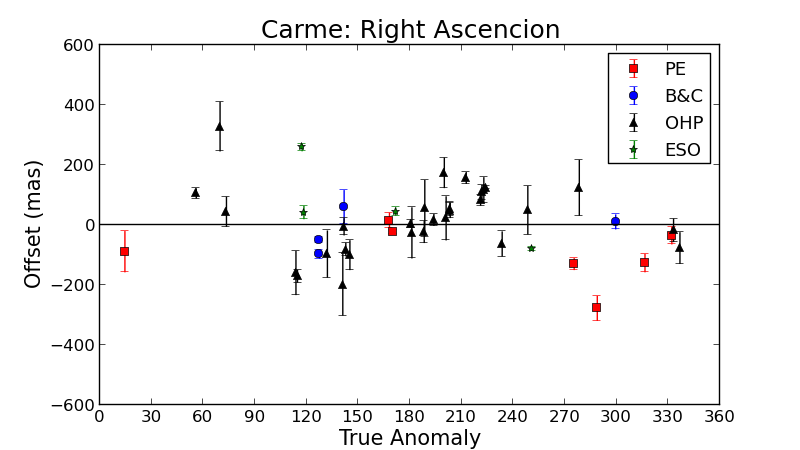
\includegraphics[scale=0.5]{figures/Carme_RA}\label{Fig: carme_alfa}}
\subfigure[Declination]{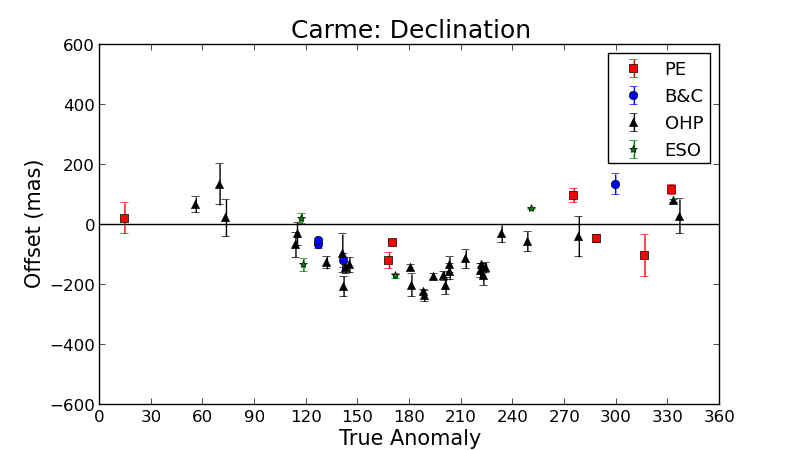
\includegraphics[scale=0.5]{figures/Carme_DEC}\label{Fig: carme_delta}}
\caption{Mean ephemeris offsets and dispersions (1 sigma error bars) in the coordinates of Carme taken night by night by true anomaly for each telescope. \textbf{The red square is for the observations with the Perkin-Elmer telescope from OPD, the blue circle for Boller \& Chivens, the magenta triangle down for Zeiss, the black triangle up for OHP and the green star for ESO.}}
\label{Fig: carme_anom}
\end{centering}
\end{figure*}

\begin{figure*}
\begin{centering}
\subfigure[Right Ascension]{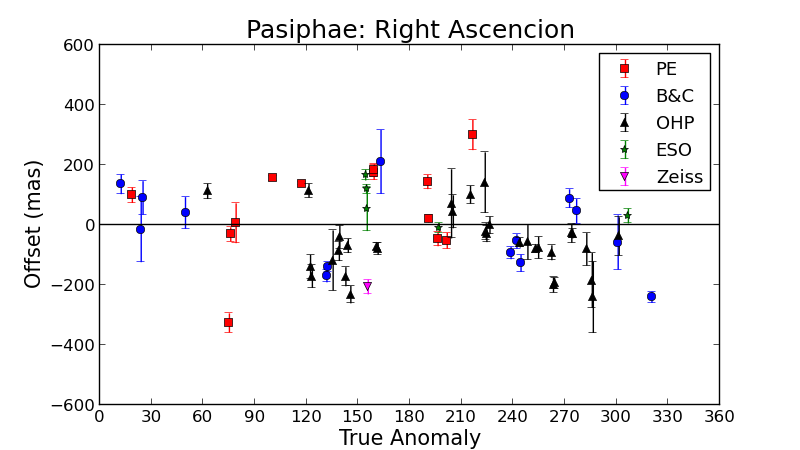
\includegraphics[scale=0.5]{figures/Pasiphae_RA}\label{Fig: pasiphae_alfa}}
\subfigure[Declination]{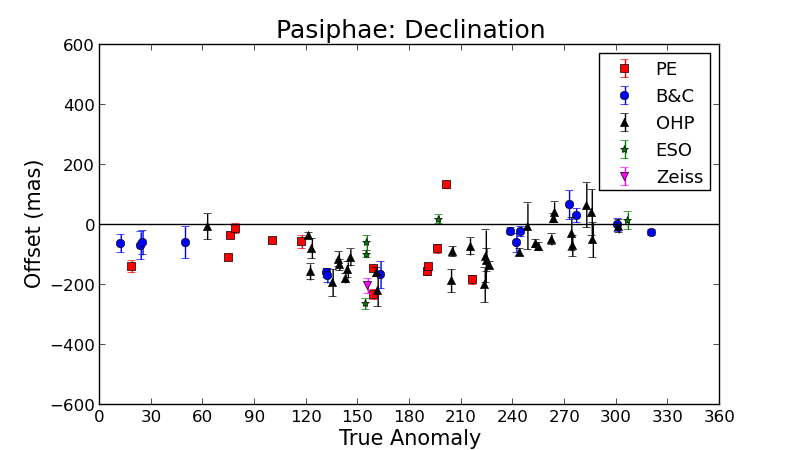
\includegraphics[scale=0.5]{figures/Pasiphae_DEC}\label{Fig: pasiphae_delta}}
\caption{Same as in Fig \ref{Fig: carme_anom} for Pasiphae.}
\label{Fig: pasiphae_anom}
\end{centering}
\end{figure*}


This pattern in declination was also seen for other satellites like Pasiphae (Fig: \ref{Fig: pasiphae_anom}) and Ananke (plots for other satellites with significant number of observations can be seen in the online material). For some satellites, the orbital coverage is not enough to clearly indicate the presence of systematic errors in specific orbital elements. However, comparing the internal position mean errors of the reductions (Table \ref{Tab: stars-errors}) with the external position errors estimated from the dispersion of the ephemeris offsets (Tables \ref{Tab: Reductions-160} to \ref{Tab: Reductions-eso}), we see position error values much larger than expected from the mean errors. This means that besides some expected astrometric errors, significant ephemeris errors must also be present.

\section{Conclusions} \label{Sec: conclusions}

\textbf{We managed a large database with FITS images acquired by 5 telescopes in 3 sites between 1992 and 2014. From that, we identified 8466 observations of irregular satellites, from which we managed to obtain 6523 suitable astrometric positions, giving a total of 3666 positions for 12 satellites of Jupiter, 1920 positions for 4 satellites of Saturn, 35 positions for Sycorax (Uranus) and 902 positions for Nereid (Neptune).}

\textbf{The positions of all the objects were determined using the PRAIA package. The package was suited to cope with the huge amount of observations and the task of identifying the satellites within the database. PRAIA tasks were also useful to deal with the missing or incorrect coordinate and time stamps present mostly in the old observations.}

\textbf{The UCAC4 was used as the reference frame. Based in the comparisons with ephemeris, we estimate that the position errors are about 60 mas to 80 mas depending on the satellite brightness. }

For some satellites the number \textbf{of positions obtained in this work} is comparable to the number used in the numerical integration of orbits by the JPL \citep{Jacobson2012} (see Table \ref{Tab: comparison-horizons}). \textbf{For instance, the amount of new positions for Himalia is about 70\% of the number used in the numerical integation of orbits by JPL}. Systematic errors in the ephemeris were found for at least some satellites (Ananke, Carme, Elara and Pasiphae). In the case of Carme, we evidenced an error in the orbital inclination \textbf{(see Fig. \ref{Fig: carme_anom})}. 

\textbf{The positions derived in this work can be used in new orbital numerical integrations, generating more precise ephemerides. Stellar occultations by irregular satellites could then be better predicted. Based in this work, our group has already computed occultation predictions for the 8 major irregular satellites of Jupiter. These predictions will be published in a forthcoming paper.}


\begin{acknowledgements}

ARGJ thanks the financial support of CAPES. M. A. thanks the CNPq (Grants 473002/2013-2 and 308721/2011-0) and FAPERJ (Grant E-26/111.488/2013). RVM thanks grants: CNPq-306885/2013, Capes/Cofecub-2506/2015, Faperj/PAPDRJ-45/2013. J-E.A. thanks the "Programme National de Planétologie" of INSU-CNRS-CNES for its financial support. J.I.B. Camargo acknowledges CNPq for a PQ2 fellowship (process number 308489/2013-6). F.B.R. acknowledges PAPDRJ-FAPERJ/CAPES E-43/2013 number 144997, E-26/101.375/2014. B.E.M. thanks the financial support of CAPES.

\end{acknowledgements}

\bibliographystyle{aa}
\nocite{*}
\bibliography{references.bib}

\Online

\begin{appendix}

\onecolumn

\section{Ephemeris offsets as a function of true anomaly for all observed irregular satellites} \label{anexo: offsets}

The distribution of ephemeris offsets along the orbit of the satellites are shown below. The red square is for the observations with the Perkin-Elmer telescope from OPD, the blue circle for Boller \& Chivens, the magenta triangle down for Zeiss, the black triangle up for OHP and the green star for ESO. For Carme and Pasiphae see Figs. \ref{Fig: carme_anom} and \ref{Fig: pasiphae_anom} in Section \ref{Sec: comparison}.

\begin{figure}[h!]
\begin{centering}
\subfigure[Right Ascension]{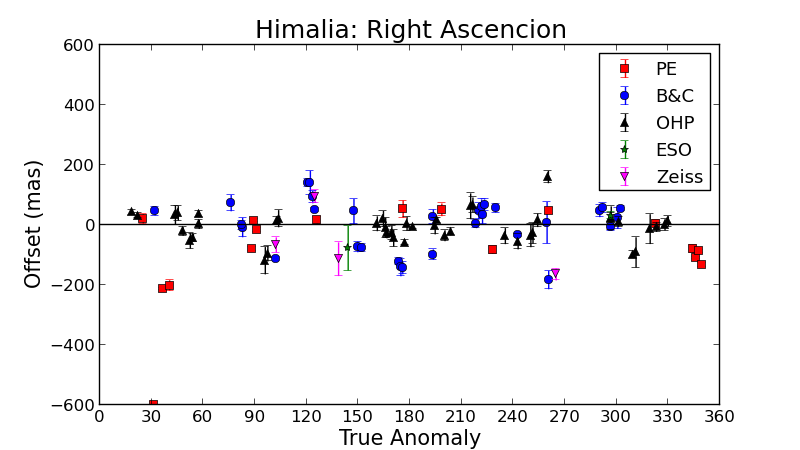
\includegraphics[scale=0.5]{figures/Himalia_RA}\label{Fig: an_himalia_alfa}}
\subfigure[Declination]{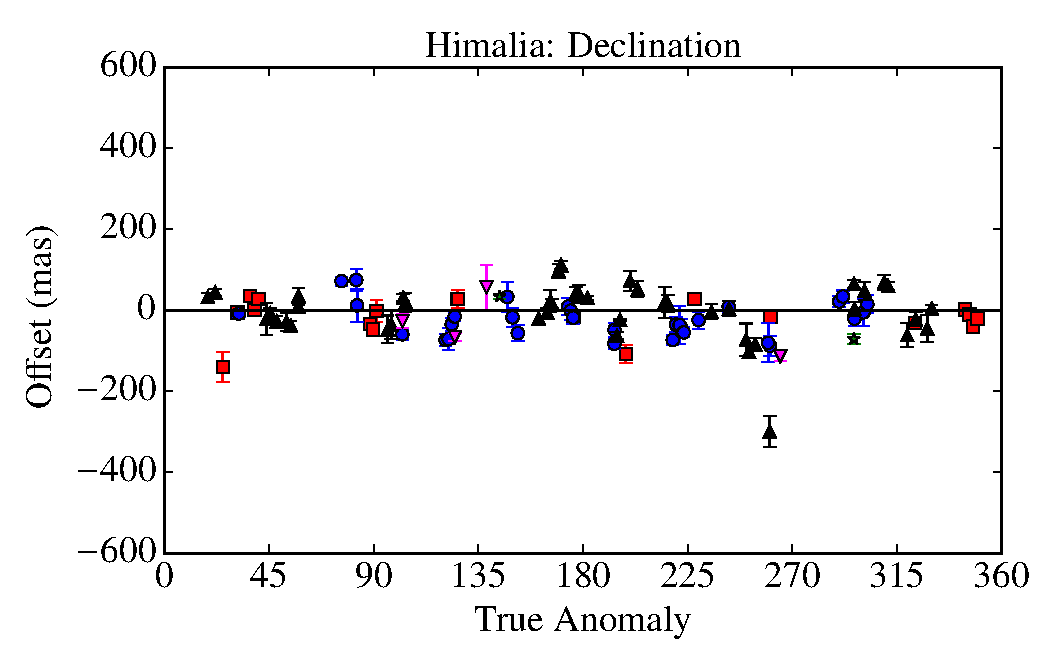
\includegraphics[scale=0.5]{figures/Himalia_DEC}\label{Fig: an_himalia_delta}}
\caption{Mean ephemeris offset and dispersion (1 sigma error bars) in the coordinates of Himalia taken night by night as a function of true anomaly.}
\label{Fig: an_himalia_anom}
\end{centering}
\end{figure}

\begin{figure}[h!]
\begin{centering}
\subfigure[Right Ascension]{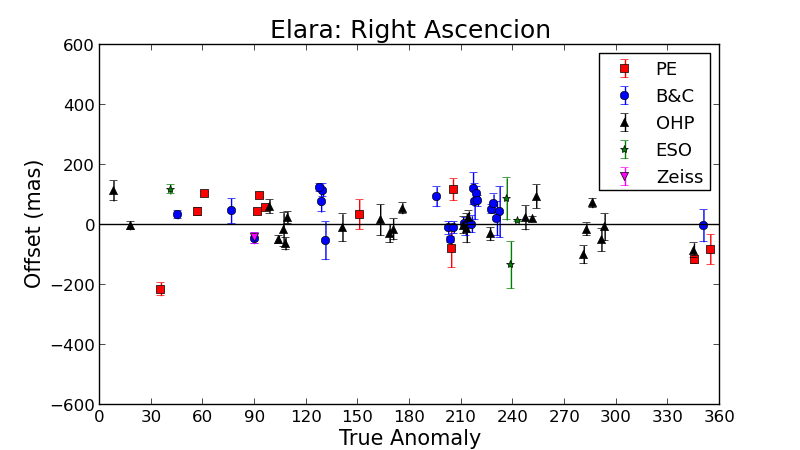
\includegraphics[scale=0.5]{figures/Elara_RA}\label{Fig: an_elara_alfa}}
\subfigure[Declination]{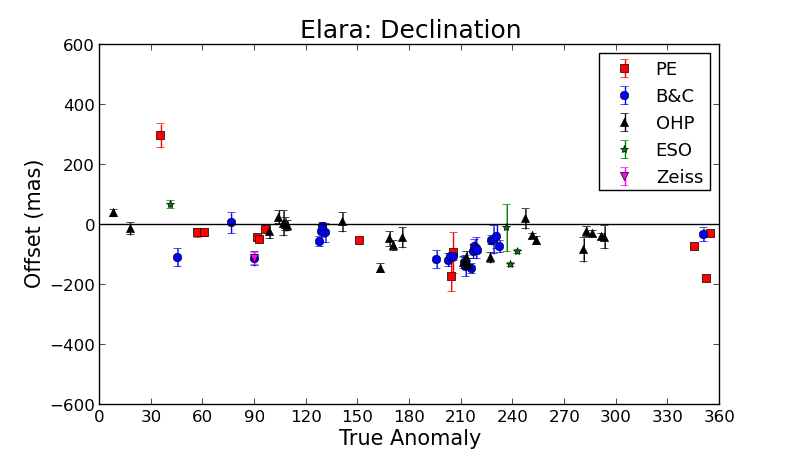
\includegraphics[scale=0.5]{figures/Elara_DEC}\label{Fig: an_elara_delta}}
\caption{Same as in Fig \ref{Fig: an_himalia_anom} for Elara.}
\label{Fig: an_elara_anom}
\end{centering}
\end{figure}

\begin{figure}[h!]
\begin{centering}
\subfigure[Right Ascension]{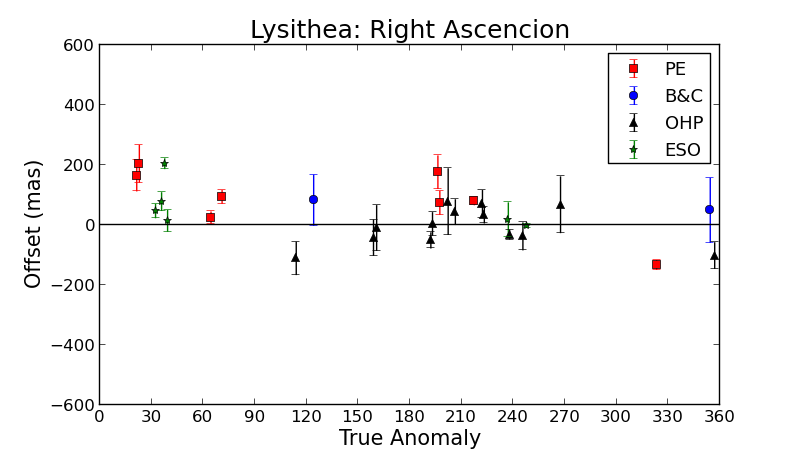
\includegraphics[scale=0.5]{figures/Lysithea_RA}\label{Fig: an_lysithea_alfa}}
\subfigure[Declination]{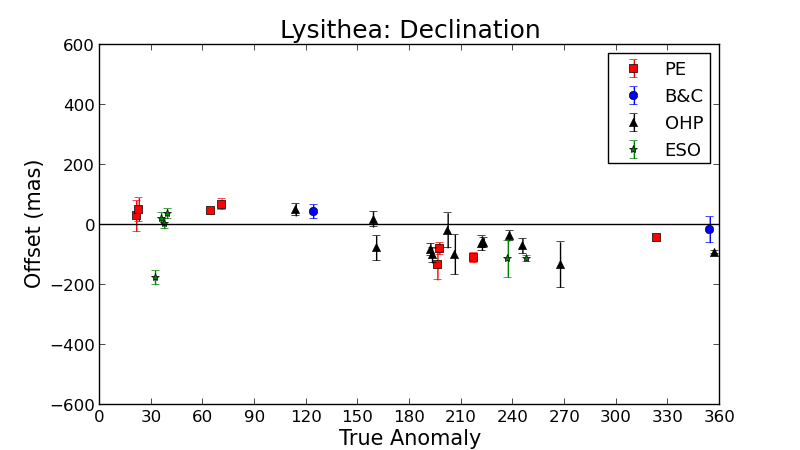
\includegraphics[scale=0.5]{figures/Lysithea_DEC}\label{Fig: an_lysithea_delta}}
\caption{Same as in Fig \ref{Fig: an_himalia_anom} for Lysithea.}
\label{Fig: an_lysithea_anom}
\end{centering}
\end{figure}

\begin{figure}[h!]
\begin{centering}
\subfigure[Right Ascension]{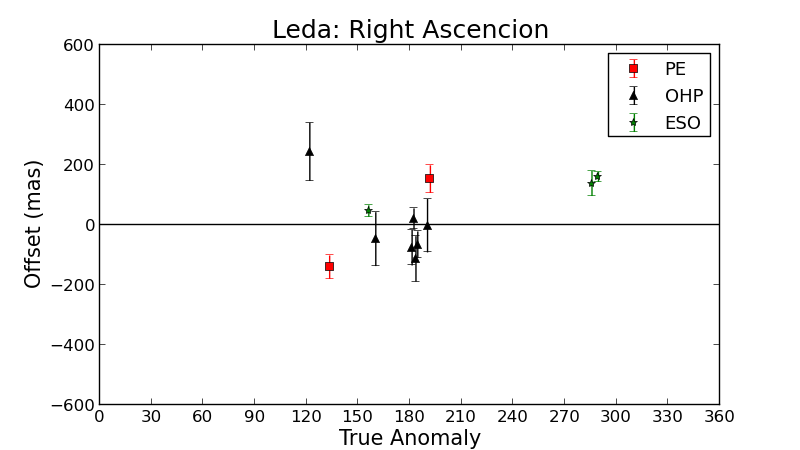
\includegraphics[scale=0.5]{figures/Leda_RA}\label{Fig: an_leda_alfa}}
\subfigure[Declination]{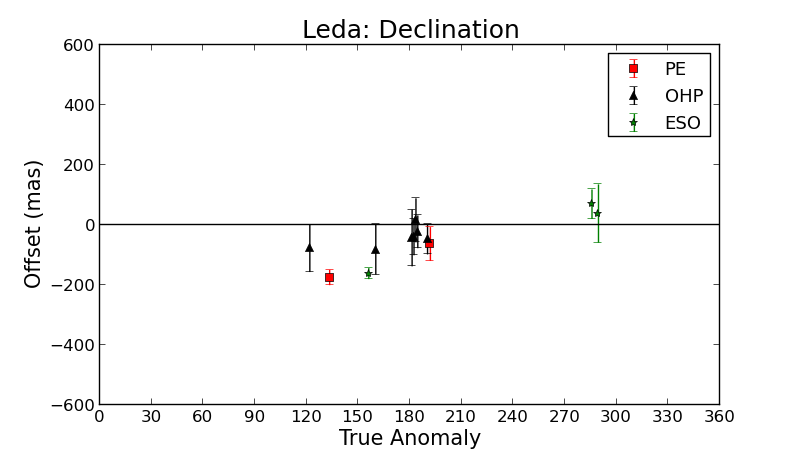
\includegraphics[scale=0.5]{figures/Leda_DEC}\label{Fig: an_leda_delta}}
\caption{Same as in Fig \ref{Fig: an_himalia_anom} for Leda.}
\label{Fig: an_leda_anom}
\end{centering}
\end{figure}

\begin{figure}[h!]
\begin{centering}
\subfigure[Right Ascension]{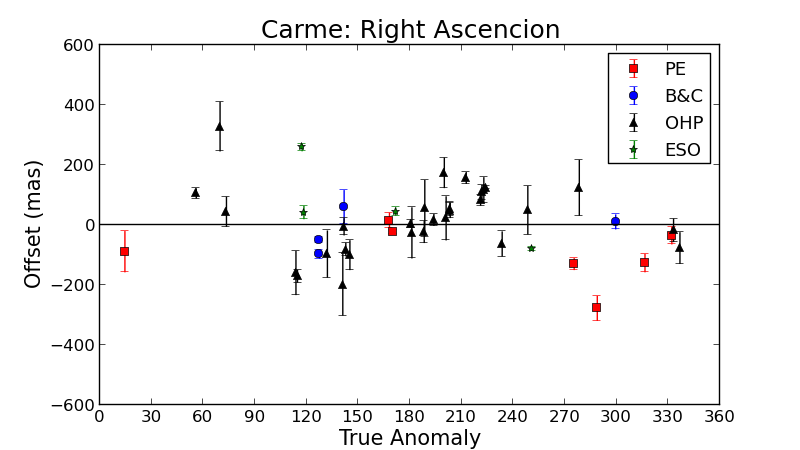
\includegraphics[scale=0.5]{figures/Carme_RA}\label{Fig: an_carme_alfa}}
\subfigure[Declination]{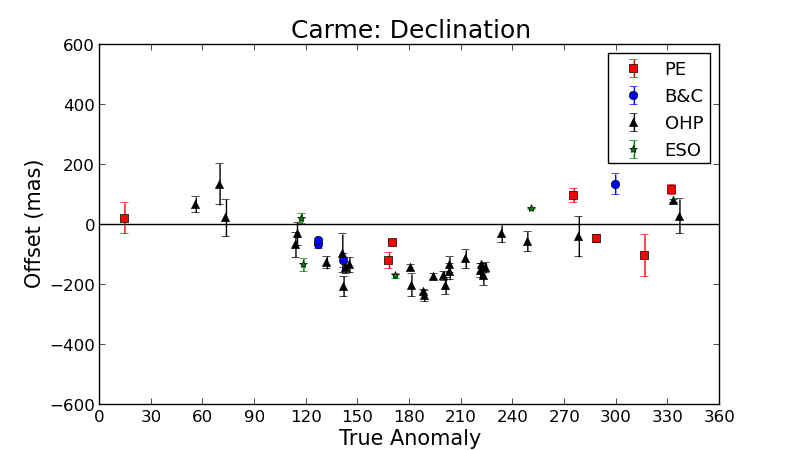
\includegraphics[scale=0.5]{figures/Carme_DEC}\label{Fig: an_carme_delta}}
\caption{Same as in Fig \ref{Fig: an_himalia_anom} for Carme.}
\label{Fig: an_carme_anom}
\end{centering}
\end{figure}

\begin{figure}[h!]
\begin{centering}
\subfigure[Right Ascension]{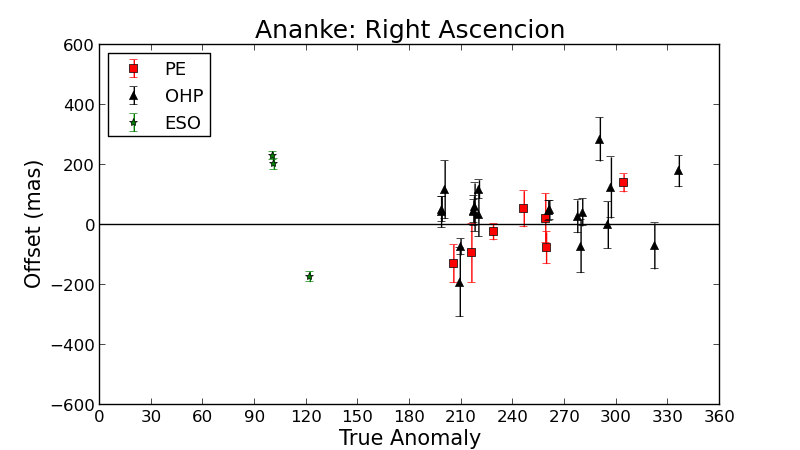
\includegraphics[scale=0.5]{figures/Ananke_RA}\label{Fig: an_ananke_alfa}}
\subfigure[Declination]{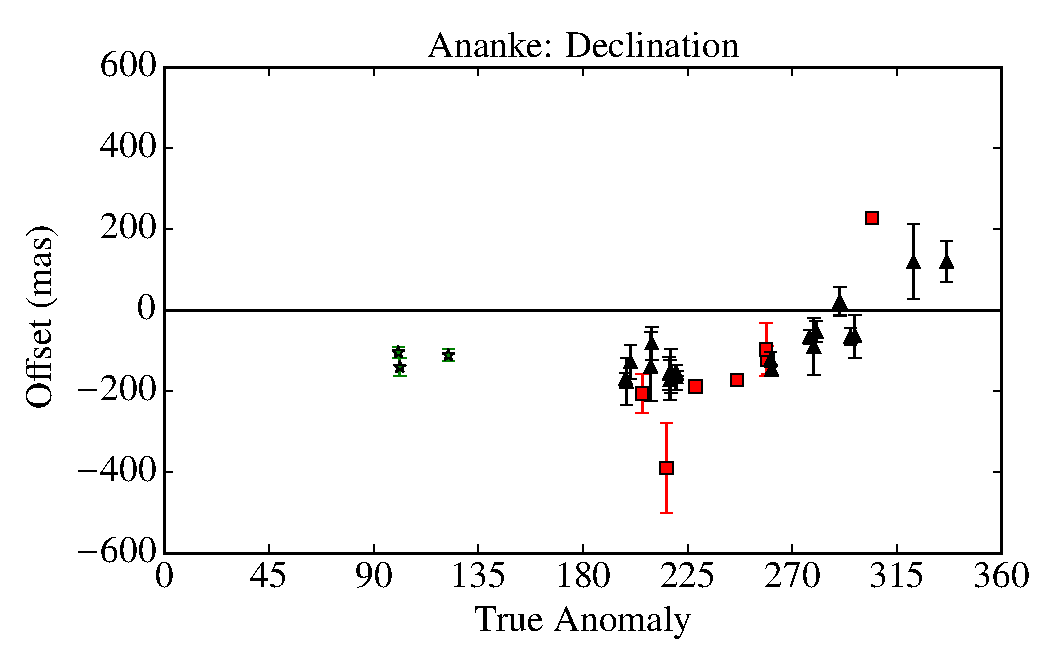
\includegraphics[scale=0.5]{figures/Ananke_DEC}\label{Fig: an_ananke_delta}}
\caption{Same as in Fig \ref{Fig: an_himalia_anom} for Ananke.}
\label{Fig: an_ananke_anom}
\end{centering}
\end{figure}




\begin{figure}[h!]
\begin{centering}
\subfigure[Right Ascension]{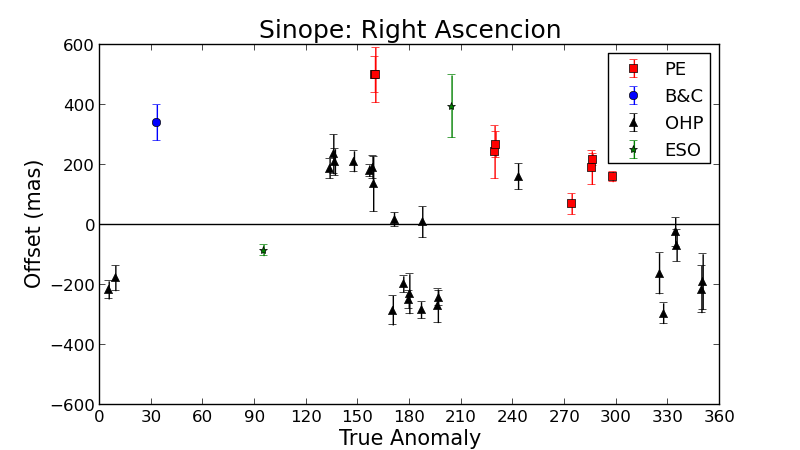
\includegraphics[scale=0.5]{figures/Sinope_RA}\label{Fig: an_sinope_alfa}}
\subfigure[Declination]{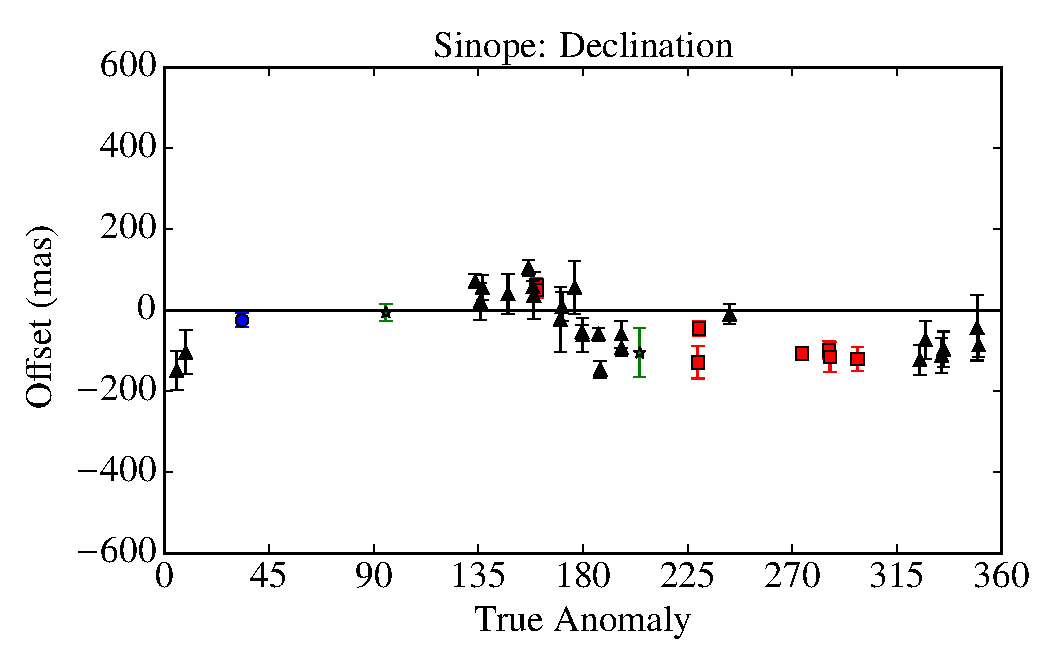
\includegraphics[scale=0.5]{figures/Sinope_DEC}\label{Fig: an_sinope_delta}}
\caption{Same as in Fig \ref{Fig: an_himalia_anom} for Sinope.}
\label{Fig: an_sinope_anom}
\end{centering}
\end{figure}

\begin{figure}[h!]
\begin{centering}
\subfigure[Right Ascension]{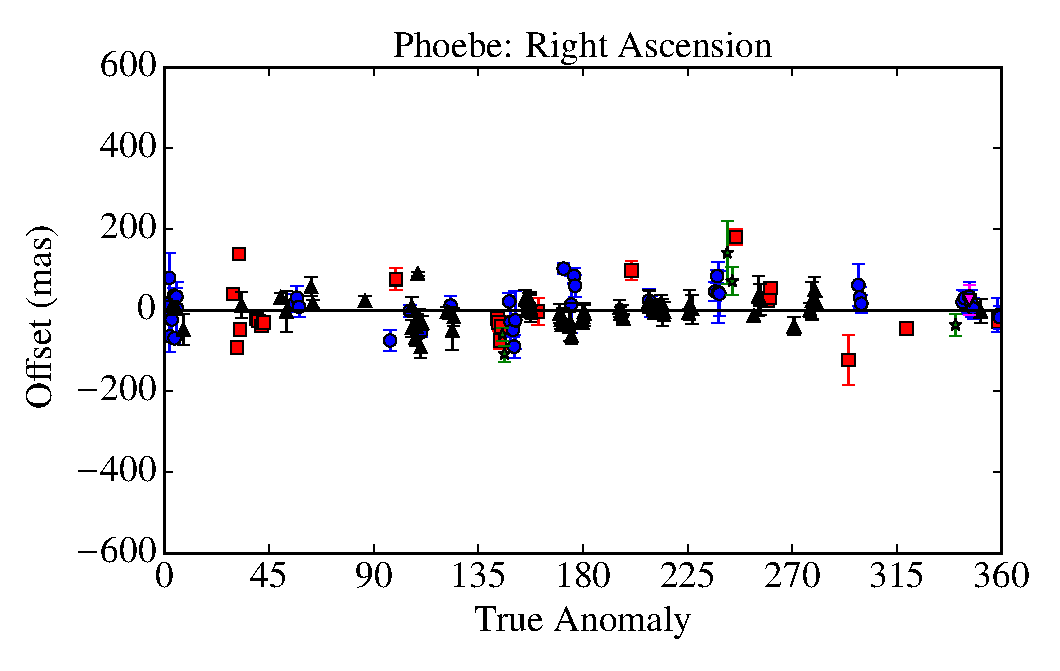
\includegraphics[scale=0.5]{figures/Phoebe_RA}\label{Fig: an_phoebe_alfa}}
\subfigure[Declination]{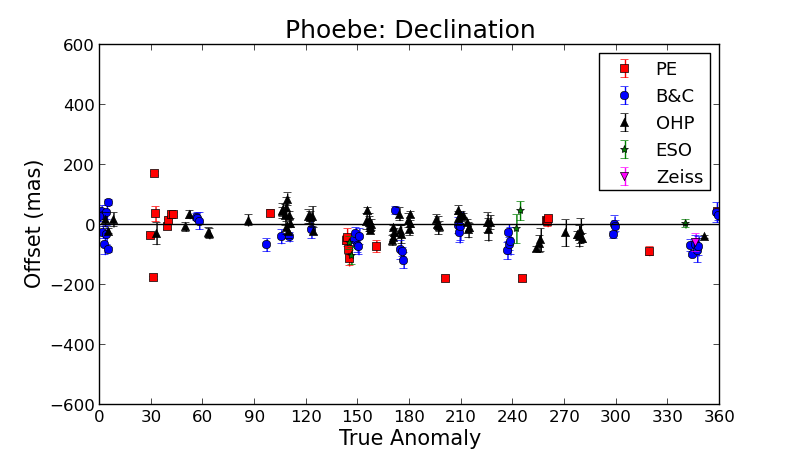
\includegraphics[scale=0.5]{figures/Phoebe_DEC}\label{Fig: an_phoebe_delta}}
\caption{Same as in Fig \ref{Fig: an_himalia_anom} for Phoebe.}
\label{Fig: an_phoebe_anom}
\end{centering}
\end{figure}

\begin{figure}[h!]
\begin{centering}
\subfigure[Right Ascension]{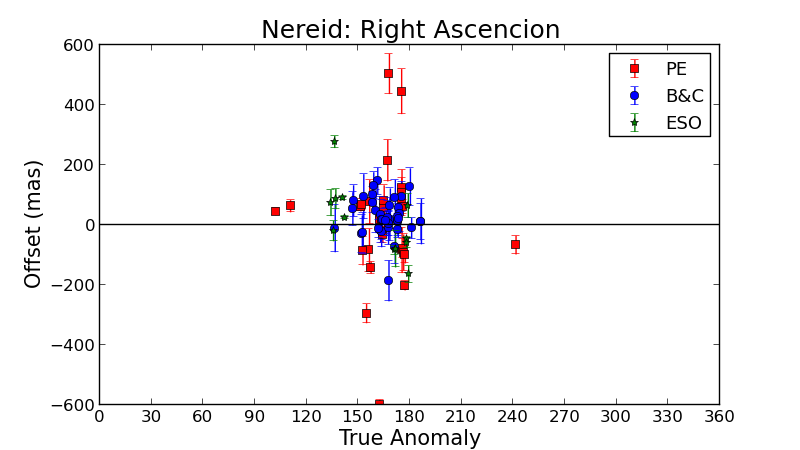
\includegraphics[scale=0.5]{figures/Nereid_RA}\label{Fig: an_nereid_alfa}}
\subfigure[Declination]{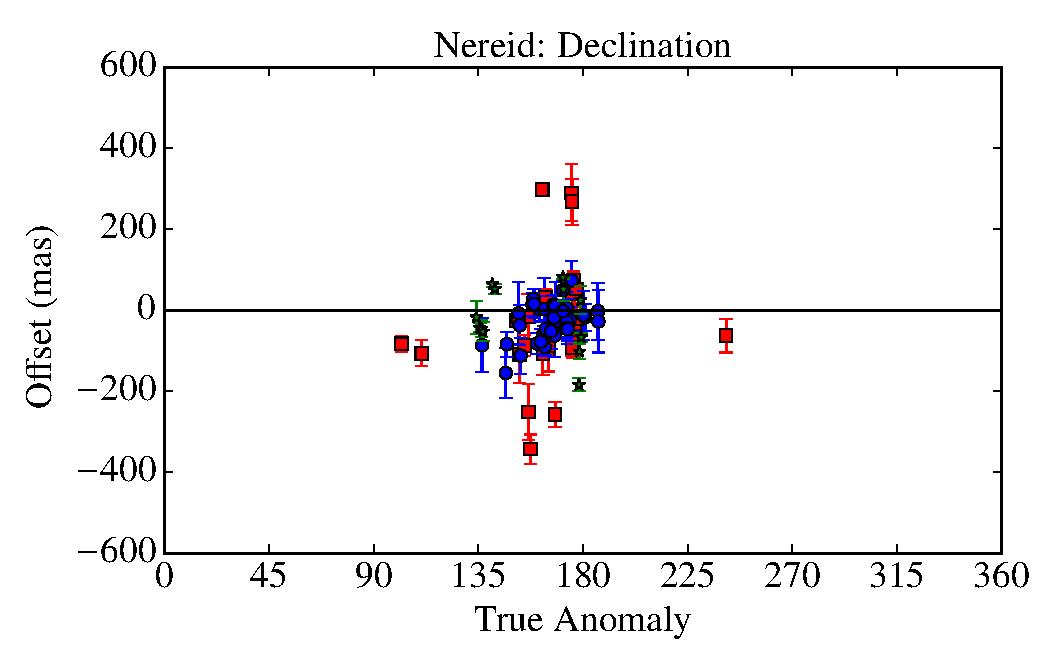
\includegraphics[scale=0.5]{figures/Nereid_DEC}\label{Fig: an_nereid_delta}}
\caption{Same as in Fig \ref{Fig: an_himalia_anom} for Nereid.}
\label{Fig: an_nereid_anom}
\end{centering}
\end{figure}


\end{appendix}


\end{document}
